\section{Упорядоченные деревья (деревья поиска). Поиск в упорядоченном дереве.  Сбалансированное дерево}
\section{Методы балансировки (самобаоансировки) деревьев}
\section{Поиск в линейных коллекциях (массивах, списках): линейный, дихотомический, поиск скачками, интерполяционный}
\section{Поиск в многомерных массивах}
\section{Нечеткий поиск - поиск подобной подстроки}
Задача нечеткого поиска (fuzzy string search)~--- найти в тексте или словаре (\textit{haystack}) все подстроки, совпадающие
(начинающиеся) с данной (\textit{needle}) с учетом не более \(k\) ошибок.
Эти алгоритмы являются основными в системах коррекции наборных ошибок
(например \href{https://en.wikipedia.org/wiki/Code_completion}{автодополнение кода} в IDE или подсказки в поисковой строке браузера).
В зависимости от преследуемых целей, существуют и используются различные алгоритмы решения данной задачи в различных постановках.

\subsubsection{Метрики Левенштейна и Хэмминга}
Расстояние Левенштейна~--- минимальное количество односимвольных операций (а именно вставки, удаления, замены),
необходимых для превращения одной последовательности символов в другую.
% cSpell: disable-next-line
Например, расстояние Левенштейна слов \(L(Hello, Hilo) = 2\) (замена `\(e\)' \(\gets\) `\(i\)', вставка `\(l\)').

Расстояние Хэмминга~--- число позиций, в которых соответствующие символы двух слов одинаковой длины различны. Например,
% cSpell: disable-next-line
\(H(Hello, Hillo) = 1\) (замена `\(e\)' \(\gets\) `\(i\)').

Расстояния Хэмминга и Левенштейна, во-первых, являются метриками в математическом смысле слова, во-вторых, позволяют строго
формализовать задачу нечеткого поиска.

Расстояние Левенштейна можно вычислить на основе рекуррентной формулы \[L(a,b) = \begin{cases}
    |a|                                  & \text{если}~|b| = 0,                         \\
    |b|                                  & \text{если}~|a| = 0,                         \\
    L(\text{tail}(a), \text{tail}(b))    & \text{если}~\text{head}(a) = \text{head}(b), \\
    1 + \min \begin{cases}
               L(\text{tail}(a), b)              \\
               L(a, \text{tail}(b))              \\
               L(\text{tail}(a), \text{tail}(b)) \\
             \end{cases} & \text{иначе}                                          \\
  \end{cases}
\]

где \(\text{tail}(\overline{x_1x_2x_3\dots}) = \overline{x_2x_3\dots}\), а \(\text{head}(\overline{x_1x_2x_3\dots}) = x_1\).
Используя также мемоизацию на матрице, можно вычислить расстояние Левенштейна между любыми двумя строками длины \(n\) и \(m\) за
\(O(n\cdot m)\)~--- алгоритм \href{https://neerc.ifmo.ru/wiki/index.php?title=%D0%97%D0%B0%D0%B4%D0%B0%D1%87%D0%B0_%D0%BE_%D1%80%D0%B5%D0%B4%D0%B0%D0%BA%D1%86%D0%B8%D0%BE%D0%BD%D0%BD%D0%BE%D0%BC_%D1%80%D0%B0%D1%81%D1%81%D1%82%D0%BE%D1%8F%D0%BD%D0%B8%D0%B8,_%D0%B0%D0%BB%D0%B3%D0%BE%D1%80%D0%B8%D1%82%D0%BC_%D0%92%D0%B0%D0%B3%D0%BD%D0%B5%D1%80%D0%B0-%D0%A4%D0%B8%D1%88%D0%B5%D1%80%D0%B0}{Вагнера-Фишера}.

\subsubsection{Алгоритм bitap}
Алгоритм \href{https://en.wikipedia.org/wiki/Bitap_algorithm}{bitap} позволяет эффективно с точки зрения реального времени работы процессора вычислять расстояние Хэмминга и
(с модификациями) Левенштейна. При асимптотике \(O(k\cdot n)\), он работает ощутимо быстрее наивного вычисления метрики
Левенштейна для сравнения двух строк, поскольку сравнивает по 32/64 символа за раз. Фактически, это эффективное
распараллеливание наивного линейного алгоритма.

\subsubsection{Алгоритм расширенной выборки}
\begin{center}
  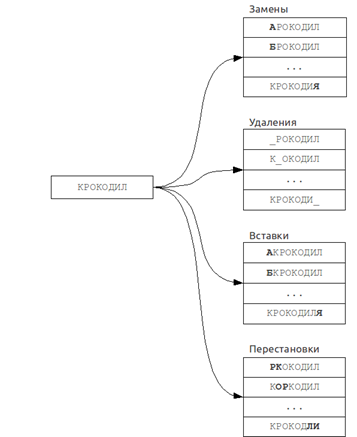
\includegraphics[width=0.3\textwidth]{resources/19-26/inflate.png}
\end{center}
Сводит задачу нечеткого поиска к задаче точного поиска последовательным перебором всех ошибочных трансформаций входной строки.
Неэффективен на больших алфавитах и при больших \(k\), даже при бинарном поиске по словарю временная сложность
\(O((m\cdot |\Sigma|)^k\cdot m\cdot \log{n})\), где \(|\Sigma|\)~--- размер алфавита.

\subsubsection{Метод \(N\)-грамм}
\begin{center}
  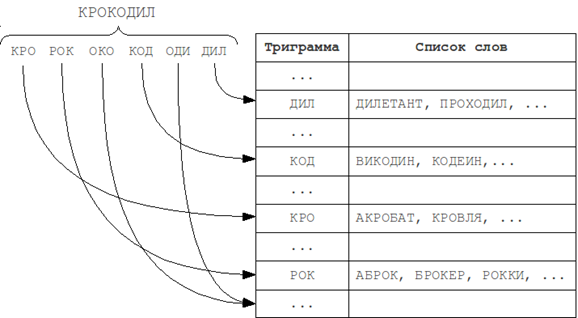
\includegraphics[width=0.3\textwidth]{resources/19-26/n-gramms.png}
\end{center}

Основан на разбиении всех слов в словаре и исходного на \(N\)-граммы~--- последовательности длины \(N\) (обычно \(N = 3\)).
\(N\)-граммы используются для группировки слов в корзины, по которым в дальнейшем и производится поиск.

\subsubsection{\href{https://cs.msu.ru/sites/cmc/files/docs/boycov.pdf}{Хеширование по сигнатуре}, \href{https://en.wikipedia.org/wiki/Locality-sensitive_hashing\#Bit_sampling_for_Hamming_distance}{Locality-sensitive hashing}}

\begin{center}
  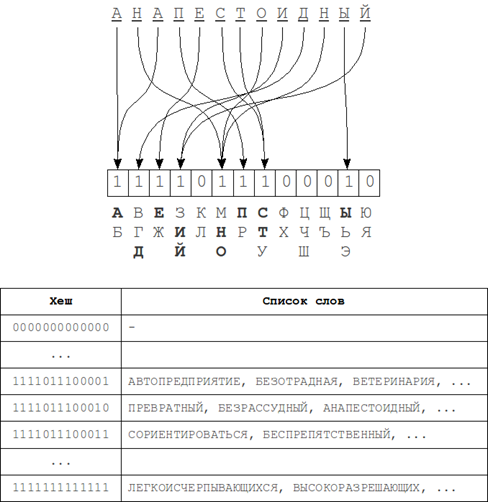
\includegraphics[width=0.3\textwidth]{resources/19-26/hash.png}
\end{center}
Предполагают сопоставление каждому слову специального хеша так, что схожие слова имеют схожие хеш-функции. Тогда поиск следует вести с
теми словами в словаре, у которых близкий или одинаковый хеш с исходной строкой.
\section{Методы сортировки (для линейных коллекций): сортировка вставкой (включением), выбором (выделением), обменом}
\section{Методы сортировки (для линейных коллекций): сортировка слиянием, "быстрая" сортировка Хоара (quicksort)}
\subsection{QuickSort (быстрая сортировка)}
Time Complexity --- $O(n\log n)$ в среднем, $O(n^2)$
в худшем (если входной массив отсортирован в обратном порядке) случае.
Space Complexity зависит от функции разбиения (функция Хоара дает $\log n$ на стек рекурсивных вызовов).

Быстрая сортировка функционирует по принципу <<разделяй и властвуй>>.
Пусть требуется отсортировать массив из $n$ элементов $a[1\dots n]$ (обе границы включены).
На первом шаге полагаем $l=1$ и $r=n$. Далее придерживаемся следующего алгоритма:
\begin{enumerate}
  \item Вычислить индекс $q$ опорного элемента.
  \item Массив $a[l\dots r]$
  разбивается на два подмассива $a[l\dots q]$ и $a[q+1\dots r]$, таких что каждый элемент $a[l\dots q]$
  меньше или равен $a[q]$, который в свою очередь, не превышает любой элемент подмассива $a[q+1\dots r]$, то есть
  \begin{align*}
    \forall\, n <&q \quad a[n] \leq a[q] \\
    \forall\, m >&q \quad a[q] \leq a[m].
  \end{align*}
  Отметим, что на этом шаге при необходимости некоторые элементы массива переставляются местами так,
  чтобы обеспечить выполнение вышеозначенного свойства.
  \item Подмассивы $a[l\dots q]$ и $a[q+1\dots r]$ сортируются рекурсивно.
\end{enumerate}

Распространенной является функция разбиения Хоара. После выбора опорного элемента $v$
заводятся два индекса: один ($i$) пробегает массив слева направо, а другой ($j$)~--- справа налево.
Когда становится верным $a[i] \geq v \geq a[j]$, элементы $a[i]$ и $a[j]$
меняются местами. После этого просмотр массива продолжается с прежних позиций. Когда индексы,
пересекутся, алгоритм завершается.

Отметим, что в качестве опорного можно выбирать абсолютно любой элемент массива
(даже всегда первый, но при такой реализации сложность любого случая будет $\Theta(n^2)$).

Если кому-либо известен алгоритм функции разбиения, то он может злонамеренно соорудить
такой массив, на котором функция быстрой сортировки уйдет в $O(n^2)$ и/или возникнет
переполнение стека. Чтобы избежать этого, в качестве опорного можно выбирать случайный
элемент массива.

Ниже приведен алгоритм Quicksort с разбиением Хоара.
\begin{minted}{C++}
/// a - массив, который сортируется
/// l - левая граница сортируемого отрезка
/// r - правая граница
int Partition(int *a, int l, int r) {
  int v = a[l + (r - l) / 2];
  int i = l;
  int j = r;
  while (i <= j) {
    while (a[i] < v) {
      ++i;
    }
    while (a[j] > v) {
      --j;
    }
    if (i >= j) {
      break;
    }
    std::swap(a[i++], a[j--]);
  }
  return j;
}

void Quicksort(int *a, int l, int r) {
  if (l < r) {
    int q = Partition(a, l, r);
    Quicksort(a, l, q);
    Quicksort(a, q + 1, r);
  }
}
\end{minted}

\subsection{Сортировка слиянием}
Данный алгоритм также использует стратегию <<разделяй и властвуй>>, рекурсивно сортируя
поданный на вход массив следующим образом:
\begin{enumerate}
  \item Массив разделяется на два подмассива так, чтобы их длины отличались не больше,
        чем на единицу;
  \item Каждый из подмассивов сортируется по отдельности рекурсивным вызовом;
  \item Посортированные массивы объединяются в один. Первый элемент результирующего 
        массива равен наименьшему из элементов подмассивов и так далее.
\end{enumerate}

Нетрудно заметить, что такая реализация потребует $O(n)$ дополнительной памяти.
Существует реализация сортировки слиянием, которая не требует дополнительной памяти,
однако она имеет большую временную сложность: $O(\log^2 n)$ против $O(\log n)$.
Ниже приведена реализация обычного алгоритма сортировки слиянием. Здесь используются
два массива, которые поочередно меняются местами. В каждом из этих массивов
в данный момент времени сортируется только одна половина исходного массива.

\begin{minted}{C++}
int *MergesortImpl(int *up, int *down, int left, int right) {
  if (left == right) {
    down[left] = up[left];
    return down;
  }

  unsigned int middle = left + (right - left) / 2;

  int *l_buff = MergesortImpl(up, down, left, middle);
  int *r_buff = MergesortImpl(up, down, middle + 1, right);

  int *target = l_buff == up ? down : up;

  unsigned int l_cur = left, r_cur = middle + 1;
  for (unsigned int i = left; i <= right; i++) {
    if (l_cur <= middle && r_cur <= right) {
      if (l_buff[l_cur] < r_buff[r_cur]) {
        target[i] = l_buff[l_cur];
        l_cur++;
      } else {
        target[i] = r_buff[r_cur];
        r_cur++;
      }
    } else if (l_cur <= middle) {
      target[i] = l_buff[l_cur];
      l_cur++;
    } else {
      target[i] = r_buff[r_cur];
      r_cur++;
    }
  }
  return target;
}

void Mergesort(int *array, int len) {
  int *back = new int[len];
  std::copy(array, array + len, back);
  int *sorted = MergesortImpl(array, back, 0, len - 1);
  if (sorted != array) {
    std::copy(back, back + len, array);
  }
  delete[] back;
}
\end{minted}